\documentclass{article}
\usepackage[utf8]{inputenc}
\usepackage{geometry}
%\usepackage{polski}
\usepackage{float}
\usepackage{graphicx}
\usepackage[shortlabels]{enumitem}
\usepackage{amsmath}
\usepackage{amsthm}
\usepackage{amsfonts}
\usepackage{amssymb}
\usepackage{hyperref}
\usepackage{array}

\usepackage{xcolor}
\usepackage{indentfirst}
\usepackage{caption}
\usepackage{subcaption}
\title{Report 1}
\author{Aleksander Jakóbczyk i Bogdan Banasiak\\ 
	Index number: 255939 i 256456}
\date{}\date{}

\newtheorem{theorem}{Theorem}
\newtheorem{definition}{Definition}

\DeclareMathOperator{\sign}{sign}
\renewcommand{\thesubsubsection}{\thesubsection. \roman{subsubsection})}

\begin{document}
	
	\maketitle
	%\section*{title}
	\section{Information and formulas}
		\subsection*{Stable random variable}
		There are two parameterizations of a random variable from an alpha stable distribution $S(\alpha, \beta , \gamma, \delta; 0)$ and $S(\alpha, \beta , \gamma, \delta; 1)$.
		They are uniquely determined by the characteristic function.
		\begin{definition} A random variable $X$ is stable if and only if $X=^d aZ +b$, with \\$\alpha \in (0,2],\;\beta\in [-1,1],\; a\ne1,\; b\in\mathbb{R}$ and $Z$ is a random variable with characteristic function  
			\begin{gather*}
				\varphi_Z(u) = \exp(i u Z) =
				\begin{cases}\label{def:case Z}
					\exp\left(- |u|^\alpha(1-i\beta\tan(\frac{\pi\alpha}{2})(\sign u)  \right) &\alpha \ne 1,\\
					\exp\left(- |u|^\alpha(1+i\beta\frac{2}{\pi}(\sign u)\ln|u|  \right) &\alpha = 1.
				\end{cases}
			\end{gather*}
		\end{definition}
		\begin{definition} Let $X \sim S(\alpha, \beta , \gamma, \delta; 0)$ with $\alpha \in (0,2]$, $\beta \in [-1,1]$, $\gamma \ge 0$, $\delta\in\mathbb{R}$ then  
			\begin{gather*}
				X \stackrel{d}{=} 
				\begin{cases}
					\gamma (Z- \beta\tan(\frac{\pi\alpha}{2})+\delta)& \alpha\ne1,\\
					\gamma Z + \delta& \alpha=1,
				\end{cases}
			\end{gather*}
			where $Z = Z(\alpha,\beta)$ is given by \ref{def:case Z}. $X$ has characteristic function
			\begin{gather*}
				E \exp (i u X)= \begin{cases}
					\exp \left(-\gamma^\alpha|u|^\alpha\left[1+i \beta\left(\tan \frac{\pi \alpha}{2}\right)(\operatorname{sign} u)\left(|\gamma u|^{1-\alpha}-1\right)\right]+i \delta u\right) & \alpha \neq 1 \\ \exp \left(-\gamma|u|\left[1+i \beta \frac{2}{\pi}(\operatorname{sign} u) \log (\gamma|u|)\right]+i \delta u\right) & \alpha=1
				\end{cases}
			\end{gather*}
		\end{definition}

		\begin{definition} Let $X \sim S(\alpha, \beta , \gamma, \delta; 1)$ with $\alpha \in (0,2]$, $\beta \in [-1,1]$, $\gamma \ge 0$, $\delta\in\mathbb{R}$ then  
			\begin{gather*}
				X \stackrel{d}{=} 
				\begin{cases}
					\gamma Z + \delta & \alpha \ne 1,\\
					\gamma Z + (\delta + \beta\frac{2}{\pi}\ln\gamma)& \alpha = 1,
				\end{cases}
			\end{gather*}
			where $Z = Z(\alpha,\beta)$ is given by \ref{def:case Z}. $X$ has characteristic function
			
			\begin{gather*}
				E \exp (i u X)= 
				\begin{cases}
					\exp \left(-\gamma^\alpha|u|^\alpha\left[1-i \beta\left(\tan \frac{\pi \alpha}{2}\right)(\operatorname{sign} u)\right]+i \delta u\right) & \alpha \neq 1 \\ \exp \left(-\gamma|u|\left[1+i \beta \frac{2}{\pi}(\operatorname{sign} u) \log |u|\right]+i \delta u\right) & \alpha=1
				\end{cases}
			\end{gather*}
		\end{definition}

		Above we defined the general stable law in the 0-parameterization and 1-parameterization.
		Alternatively, we can swap between the parameterizations using the following theorem;
		\begin{theorem}Let $Z\sim S(\alpha,\beta,1,0;0)$  with $\alpha \in (0,2]$, $\beta \in [-1,1]$, $\gamma \ge 0$, $\delta\in\mathbb{R}$ then  
			\begin{gather*}
				\begin{cases}
					\gamma Z + \delta + \beta \gamma \tan\left(\frac{\pi\alpha}{2}\right) &\alpha\ne1,\\
					\gamma Z + \delta + \beta \frac{2}{\pi}\ln\gamma  &\alpha=1
				\end{cases}\sim S(\alpha,\beta,\gamma,\delta; 1),
			\end{gather*}
		\end{theorem}

		The tail exponent estimation method gives us the information
		about the index of stability. The tails of stable random variable are asymptotically power laws. 
		\begin{theorem}[Tail approximation] Let $X \sim S(\alpha, \beta , \gamma, \delta; k)$ with $\alpha \in (0,2)$, $\beta \in (-1,1]$, $k=0,1$ then as~$x\to \infty$:
			\label{theorem:Tail approximation}
			\begin{align*}
				1 - F_X(x) &\sim \gamma^\alpha c_a (1+\beta)x^{-\alpha},\\
				f_X(x) &\sim \alpha \gamma^\alpha c_a (1+\beta) x^{-(\alpha + 1)}
			\end{align*}
			where $c_a = \sin(\frac{\pi\alpha}{2})\Gamma(\alpha)/\pi$ and $f(x)\sim g(x)$ as $x\to a$ means $\lim_{x\to a} h(x)/f(x) = 1$. Using the reflection property, the lower tail properties are
			similar: for $\beta\in[-1,1)]$ as $x \to \infty$:
			\begin{align*}
				F_X(-x) &\sim  \gamma^\alpha c_a (1-\beta)x^{-\alpha},\\
				f_X(-x) &\sim  \alpha \gamma^\alpha (1-\beta)c_a x^{-(\alpha + 1)}
			\end{align*}
		\end{theorem}
		It follows from the above theorem that for $x\to\infty$
		\begin{gather}\label{Tail approximation polifit}
			1 - F(x) \sim Cx^{-\alpha} \implies \ln(1-F(x)) \sim \ln(C) -\alpha \ln(x)
		\end{gather}

		\begin{theorem}  Let $X \sim S(\alpha, \beta , \gamma, \delta; k)$ wwith $\alpha \in (0,2]$, $\beta \in [-1,1]$, $\gamma \ge 0$, $\delta\in\mathbb{R}$, $k=0,1$ then
			\label{theorem:CF}
			\begin{align*}
				|\varphi_X(u)| &= e^{-C|u|^\alpha} \implies \\
				\ln |\varphi_X(u)| &= -C|u|^\alpha \implies \\
				\ln(-\ln |\varphi_X(u)|) &= \ln(C) + \alpha\ln|u|
			\end{align*}
		\end{theorem}
		Theorems \ref{theorem:Tail approximation} and \ref{theorem:CF} allows us to determine the stability index using linear regression.

		\begin{definition}Let $X_1,\dots, X_n$ be i.i.d. random variables with the common cumulative distribution function $F(t)$. 
			Then the empirical distribution function is defined as
			\begin{gather*}
				\hat{F_n}(x) = \frac{1}{n}\sum_{k = 1}^{n}\mathbf{1}_{\{X_k \le x\}}
			\end{gather*}
		\end{definition}
		\begin{definition}Let $X_1,\dots, X_n$ be i.i.d. random variables with the characteristic function $\varphi(t)$. 
			Then the empirical characteristic function is defined as
			\begin{gather*}
				\hat{\varphi_n}(u) = \frac{1}{n}\sum_{k = 1}^{n}e^{-i u X_k}
			\end{gather*}
		\end{definition}
		\section{Compare two estimators of $\alpha$ parameter we introduced in the laboratories}

		We will be conducting our simulations on consider one set of parameters $(\alpha, \beta , \gamma, \delta) = (1.5, 0.8, 2, 0)$.

		\subsection{Based on the ECDF}
		\subsubsection{}
		We gernerated $n = 10^6$ samples of alfa-stable distribution.
		A figure \ref{stable_cdf} depicts cumulative distribution function of theoretical variable (blue) compared to generated one (orange).
		Based on this graph  and the KS test $p\text{-value} = 0.14623$ we do not reject the hypothesis of different distributions and assume that the program that generates the variables is working correctly.
		
		Graph at the right side shows CDF for higher values of $x$, thanks to which we can use the first method of estimation parameter $\alpha$ based on theorem \ref{theorem:Tail approximation} and properties \ref{Tail approximation polifit}.    
		
		\begin{figure}[H]	
			\begin{subfigure}[h]{.5\textwidth}
				\centering
				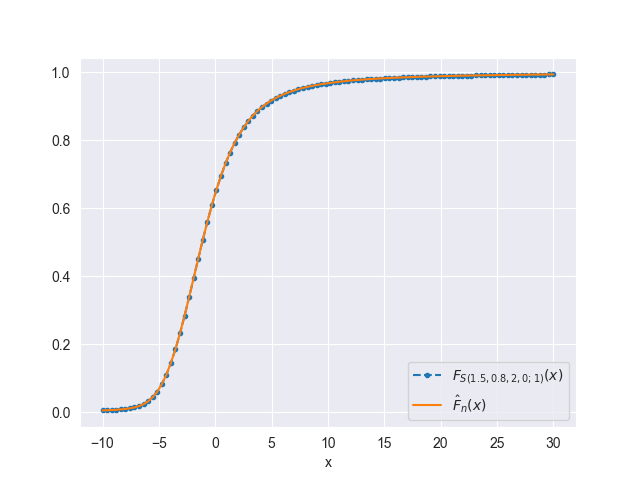
\includegraphics[width=1\linewidth]{images/stable_CDF.png}
				\caption{CDF simulated for $x \in (-10,30)$.}
			\end{subfigure}
			\begin{subfigure}[r]{.5\textwidth}
				\centering
				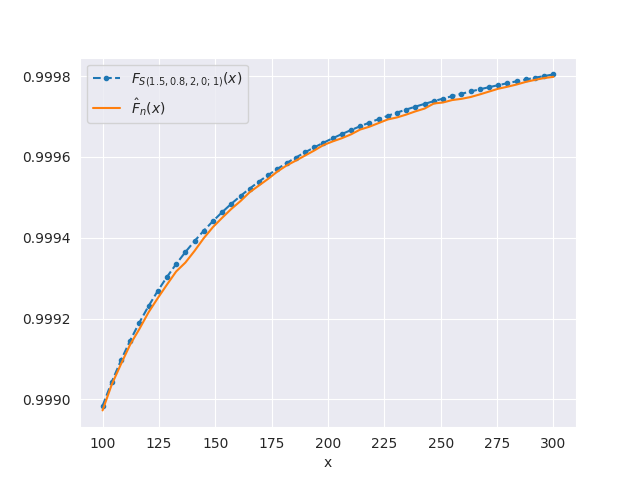
\includegraphics[width=1\linewidth]{images/stable_CDF_large_x.png}
				\caption{CDF simulated of tail for $x \in (10,30)$.}
			\end{subfigure}
			\caption{CDF of a random variable with an $\alpha$-stable distribution based on $n=10^6$ realizations of the random variable.}\label{stable_cdf}
		\end{figure}

		Following the first method, using logarithm of distribution's tail, we successfully fitted parameters to our model.
		Results are shown at figure \ref{tails1}, where blue line is a teoretical distribution, orange line represents empirical one and green is a fitted model.
		\subsubsection{}
        After checking the correctness of the method, we estimated parameter $\alpha$ using a Monte Carlo simulation with 1000 steps and 20000 samples on each step.
		Distribution of estimated parameters can be observed at figure \ref{alpha1}, where we have placed density histogram and boxplot.
		We can see, that the mean of estimation is correct, but there are also a lot of outliers.		 
		
		\begin{figure}[H]
			\centering
			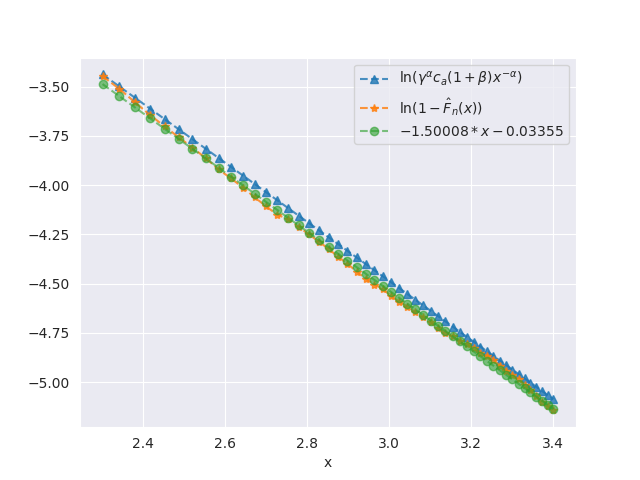
\includegraphics[width=1\linewidth]{images/compare_cdf_plots_type_1.png}
			\caption{Plot of tail approximation method fitted line.}\label{tails1}
		\end{figure}

		\begin{figure}[H]
			\begin{subfigure}{.5\textwidth}
				\centering
				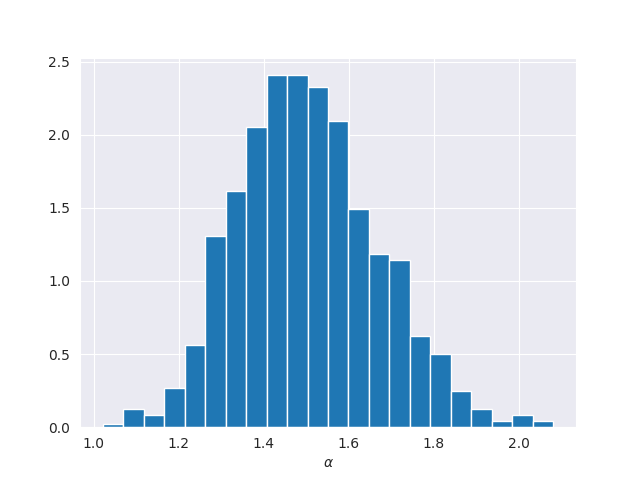
\includegraphics[width=1\linewidth]{images/cdf_alpha_hist.png}
				\caption{Histogram of the $\hat\alpha$ estimator.				}
			\end{subfigure}
			\begin{subfigure}[r]{.5\textwidth}
				\centering
				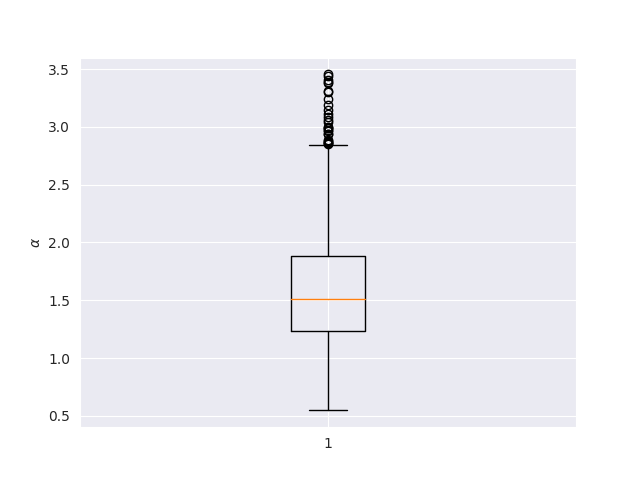
\includegraphics[width=1\linewidth]{images/cdf_alpha_boxplot.png}
				\caption{Boxplot}
			\end{subfigure}
			\caption{Distribution of the estimator of the $\alpha$ parameter based on Monte Carlo simulations for tail approximation method.}\label{alpha1}
		\end{figure}
	
		In addition, we have included basic statistics in the table \ref{tabelka1}. We can see, that the distribution of estimator has high std.  Maximal and minimal values are absolutly too far from true value of $\hat\alpha$. Skewness is equal to 0.28487 and with the analysis of the graph we assess, that distribution is right-skewed. The kurtosis is close to zero, so we can assume that it is leptokurtic distribution, so we can expect havy tails and this is correct with values of quantiles.
		
		\begin{table}[H]
			\centering
			\begin{tabular}{|c|c|c|c|c|c|c|c|c|c|}
				\hline
				count &      mean &       std &       min &     25\% &       50\% &     75\% &      max & skewness & kurtosis \\\hline
				1000 & 1.5081 &  0.1697 &  0.994552 &  1.3893 &  1.5051 &  1.6112 &  2.0974 & 0.2849 & 0.0931\\\hline
			\end{tabular}
			\caption{Table of basic statistics of the $\hat\alpha$ estimator for tail approximation method.}\label{tabelka1}
		\end{table}
		\subsubsection{}
		We checked, how selected parameters affect MSE and MAE. We made simulation of 100 steps of Monte Carlo and 5000 samples of generated $\hat\alpha$, to create adequate heatmaps.
		
		On figure \ref{heat1} we placed results for Mean Squared Error. At the left side we inserted dependencies of $\alpha$ and $\beta$ using $\gamma=2$ and $\delta=0$ and at the right side we placed dependencies of $\gamma$ and $\delta$ using $\alpha=1.5$ and $\beta=0.8$
		
		The main conclusion is, that the smaller $\beta$ we take, the worse results we obtain. The same result we get for $\alpha$. 
		
		We get smaller errors within increasing $\gamma$, but for $\delta$ we obtain the best results where it is equal to 0 and farther we go from zero, then worse. Delta should not have influance on the highest of error becouse this method uses aproximation of infinitive values, but our domain is the range from 10 to 30. We did it becouse we decided to optimalise the process of generating $\hat\alpha$, so in this case, selection of $\delta$ has big influance on the generated tails. Anyway, the differences of results depended on $\gamma$ and $\delta$ are smaller than dependent on $\alpha$ and $\beta$.
		
		\begin{figure}[H]
			\begin{subfigure}{.5\textwidth}
				\centering
				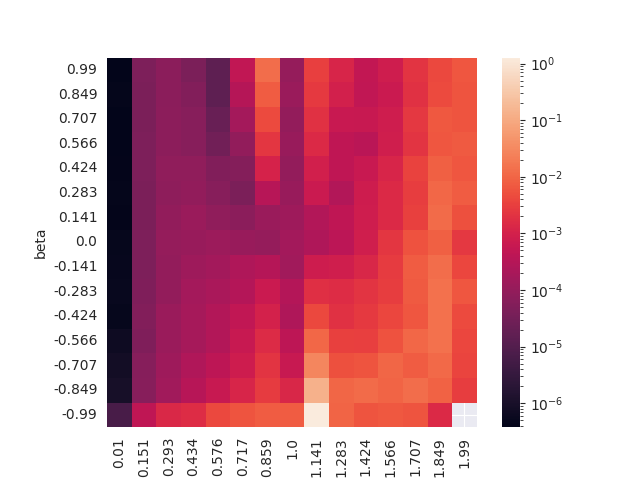
\includegraphics[width=1\linewidth]{images/heatmap_cdf_MSE_alpha_beta.png}
				\caption{Depending on $\alpha, \beta$ parameters and \\$\gamma = 2, \delta = 0$}
			\end{subfigure}
			\begin{subfigure}[r]{.5\textwidth}
				\centering
				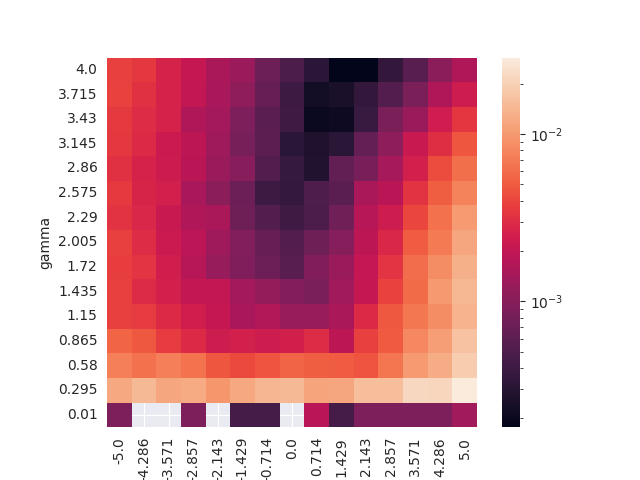
\includegraphics[width=1\linewidth]{images/heatmap_cdf_MSE_gamma_delta.png}
				\caption{Depending on $\gamma, \delta$ parameters and \\$\alpha = 1.5, \beta = 0.8$}
			\end{subfigure}
			\caption{Heatmaps of Mean Squared Error (MSE) based on Monte Carlo simulations for tail approximation method.}\label{heat1}
		\end{figure}
	
		We created also a heatmaps of MAE (figure \ref{heat2}). We used the same parameters as in the case with MSE. In this example we obtain the same dependences, but the only one difference is with the scale of errors, what is meaningful, if we would check the formula of MAE.
		
		
		\begin{figure}[H]
			\begin{subfigure}{.5\textwidth}
				\centering
				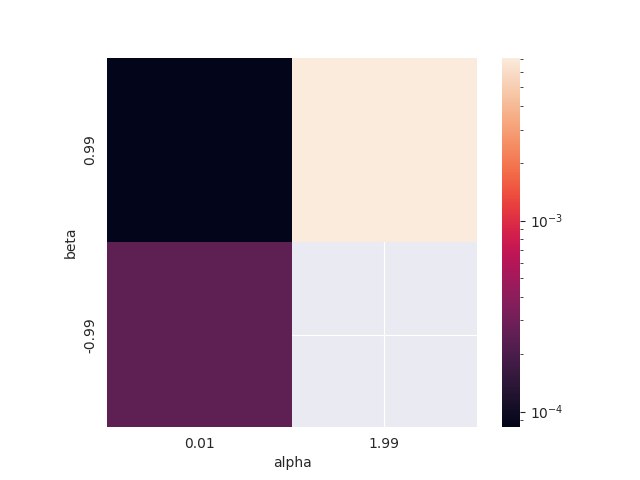
\includegraphics[width=1\linewidth]{images/heatmap_cdf_MAE_alpha_beta.png}
				\caption{Depending on $\alpha, \beta$ parameters and \\$\gamma = 2, \delta = 0$}
			\end{subfigure}
			\begin{subfigure}[r]{.5\textwidth}
				\centering
				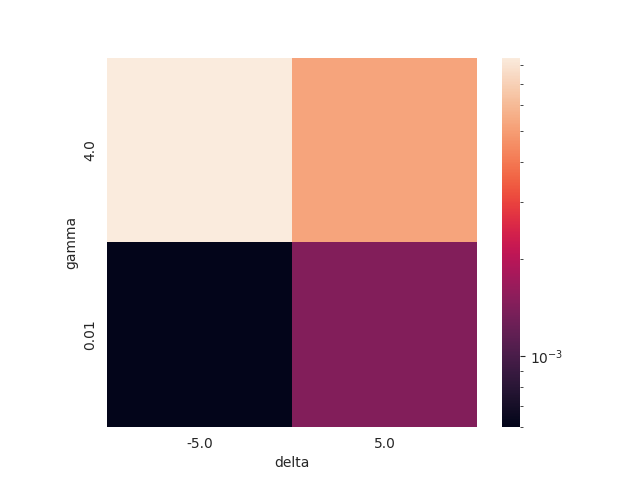
\includegraphics[width=1\linewidth]{images/heatmap_cdf_MAE_gamma_delta.png}
				\caption{Depending on $\gamma, \delta$ parameters and \\$\alpha = 1.5, \beta = 0.8$}
			\end{subfigure}
			\caption{Heatmaps of Mean Absolute Error (MAE) based on Monte Carlo simulations for tail approximation method.}\label{heat2}
		\end{figure}

		\subsection{Based on the CF}
		\subsubsection{}
		Now we will consider second method of estimation parameter $\alpha$ [\ref{theorem:CF}]. First we crated an empirical characteristic function by generating 10000 samples from alpha-stabil distribution. At figure \ref{cf1} we presented comparison of theoretical (orange line) and empirical (blue line) CF. We can see, that empirical plot is similar to theoretical one.
		
		\begin{figure}[H]
				\centering
				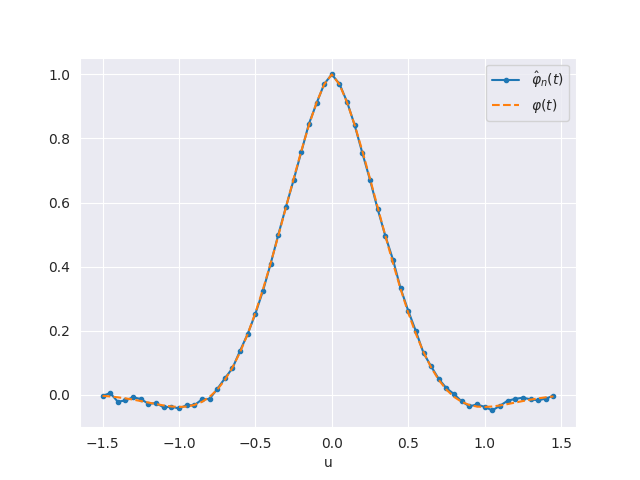
\includegraphics[width=1\linewidth]{images/stable_CF.png}
			\caption{CF of a random variable with an $\alpha$-stable distribution based on $n=10000$ realizations of the random variable for each $t$.}\label{cf1}
		\end{figure}

		Following this method, using double logarithm on CF, we successfully fitted parameters to our model. Correctness of the fitting is shown in figure \ref{CF_line2}, where blue line is theoretical function, orange in estimated one and green is a line represanting suitable model.
		
		\begin{figure}[H] 
			\centering
			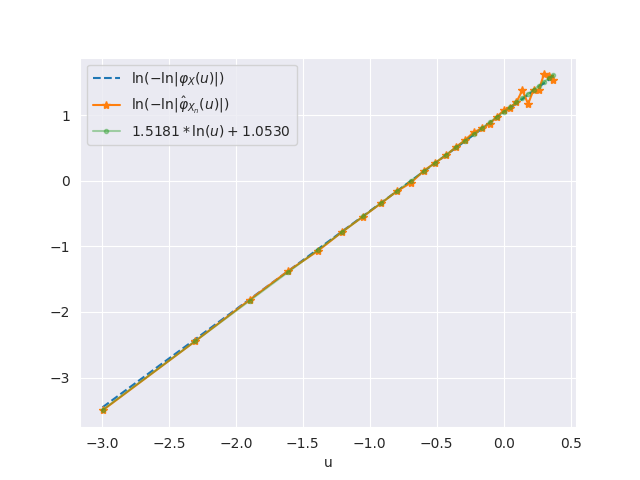
\includegraphics[width=1\linewidth]{images/compare_cf.png}
			\caption{Plot of characteristic function method fitted line.}\label{CF_line}
		\end{figure}
		\subsubsection{}
		
		We checked the correctness of this method by estimating parameter $\alpha$ using a Monte Carlo simulation with 1000 steps and 5000 samples on each step.
		
		Distribution of estimated parameters can be observed in figure \ref{alpha2}, where we have placed density histogram and boxplot and we have included basic statistics in the table \ref{tabelka2}.
		We can see, that the mean of estimation is correct. We obtain better std then using tail approximation method. Whatsmore, in this case, the skewness is low, close to 0. The kurtosis is equal to -0.1926, so the distribution is platokurtic.
		
		\begin{figure}[H]
			\begin{subfigure}{.5\textwidth}
				\centering
				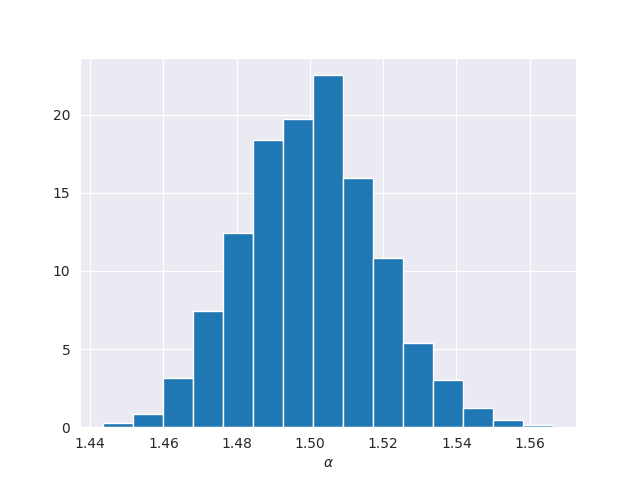
\includegraphics[width=1\linewidth]{images/cf_alpha_hist.png}
				\caption{Histogram of the $\hat\alpha$ estimator.}\label{CF_line2}
			\end{subfigure}
			\begin{subfigure}[r]{.5\textwidth}
				\centering
				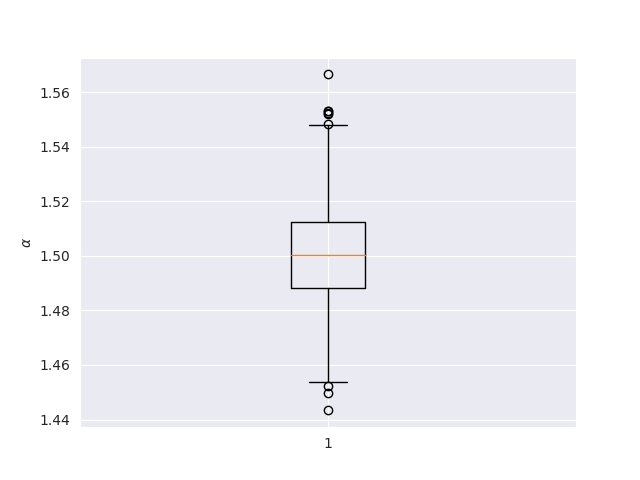
\includegraphics[width=1\linewidth]{images/cf_alpha_boxplot.png}
				\caption{Boxplot of the $\hat\alpha$ estimator.}
			\end{subfigure}
			\caption{Distribution of the estimator of the $\alpha$ parameter based on Monte Carlo simulations for characteristic function method.}\label{alpha2}
		\end{figure}
		
		\begin{table}[H]
			\centering
			\begin{tabular}{|c|c|c|c|c|c|c|c|c|c|}
				\hline
				count &      mean &       std &       min &       25\% &      50\% &     75\% & max & skewness & kurtosis
				\\\hline
				1000.0 &  1.4989 &  0.0185 &  1.4468 &  1.4868 &  1.498 &  1.5118 &  1.5543 & 0.0294 & -0.1926\\\hline
			\end{tabular}
			\caption{Table of basic statistics of the $\hat\alpha$ estimator for tail approximation method.}\label{tabelka2}
		\end{table}
	
		\subsubsection{}
		We checked, how selected parameters affect MSE and MAE. We made simulation of 100 steps of Monte Carlo and 5000 samples of generated $\hat\alpha$, to create adequate heatmaps.
		
		On figure \ref{heat3} we placed results for Mean Squared Error. At the left side we inserted dependencies of $\alpha$ and $\beta$ using $\gamma=2$ and $\delta=0$ and at the right side we placed dependencies of $\gamma$ and $\delta$ using $\alpha=1.5$ and $\beta=0.8$
		
		In this case, the dependencies are really visuable. We get bigger errors within increasing $\alpha$ and $\gamma$. Changing $\beta$ and $\delta$ has no effect on the size of the error.
		
		\begin{figure}[H]
			\begin{subfigure}{.5\textwidth}
				\centering
				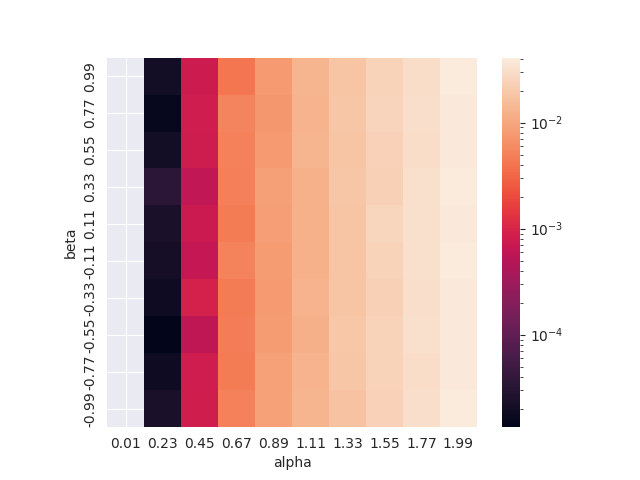
\includegraphics[width=1\linewidth]{images/heatmap_cf_MSE_alpha_beta.png}
				\caption{Depending on $\alpha, \beta$ parameters and \\$\gamma = 2, \delta = 0$}
			\end{subfigure}
			\begin{subfigure}[r]{.5\textwidth}
				\centering
				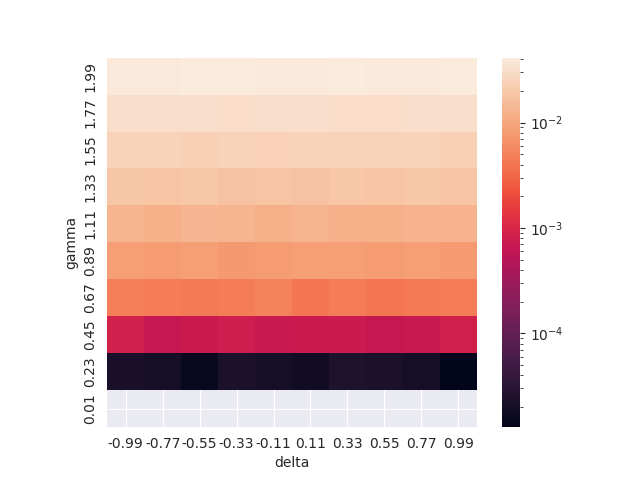
\includegraphics[width=1\linewidth]{images/heatmap_cf_MSE_gamma_delta.png}
				\caption{{Depending on $\gamma, \delta$ parameters and \\$\alpha = 1.5, \beta = 0.8$}}
			\end{subfigure}
			\caption{Heatmaps of Mean Squared Error (MSE) based on Monte Carlo simulations for characteristic function method.}\label{heat3}
		\end{figure}

		On figure \ref{heat4} we placed results for Mean Absolute Error. At the left side we inserted dependencies of $\alpha$ and $\beta$ using $\gamma=2$ and $\delta=0$ and at the right side we placed dependencies of $\gamma$ and $\delta$ using $\alpha=1.5$ and $\beta=0.8$

		The conclussion is that the size of error depend only on $\alpha$. The bigger $\alpha$, the higher error we get. High error at the bottom of right graph is coused by taking $\gamma$ to closed to 0, which is out of domain of alpha-stable distribution.

		\begin{figure}[H]
			\begin{subfigure}{.5\textwidth}
				\centering
				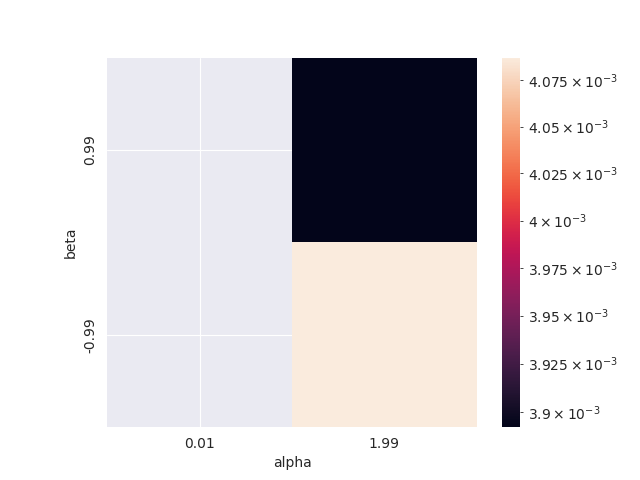
\includegraphics[width=1\linewidth]{images/heatmap_cf_MAE_alpha_beta.png}
				\caption{Depending on $\alpha, \beta$ parameters and \\$\gamma = 2, \delta = 0$}
			\end{subfigure}
			\begin{subfigure}[r]{.5\textwidth}
				\centering
				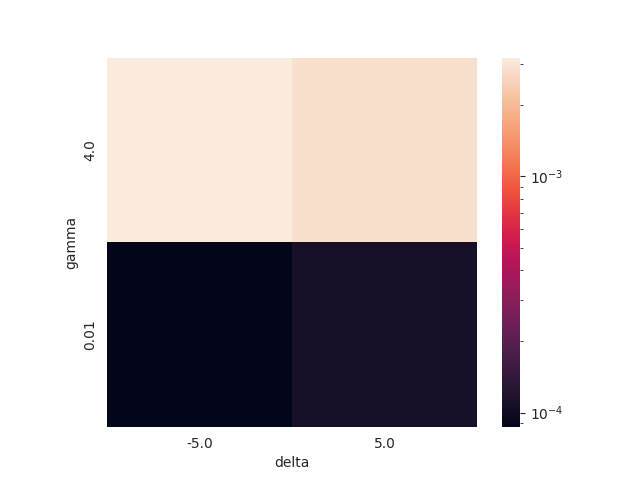
\includegraphics[width=1\linewidth]{images/heatmap_cf_MAE_gamma_delta.png}
				\caption{Depending on $\gamma, \delta$ parameters and \\$\alpha = 1.5, \beta = 0.8$}
			\end{subfigure}
			\caption{Heatmaps of Mean Absolute Error (MAE) based on Monte Carlo simulations for characteristic function method.}\label{heat4}
		\end{figure}
	
	\subsection{Summary}
	We presented the operation of both methods, which estimate parameter $\alpha$. We proved, that both of them works correctly. Errors, we obtianed by using the method which bases on characteristic function, depend strongly on parameter $\alpha$.
	 
	
\end{document}